%%%%%%%%%%%%%%%%%%%%%%%%%%%%%%%%%%%%%%%%%%%%%%%%%%%%%%%%
% Este é um documento que servirá de modelo para
% os relatórios feitos na disciplina Circuitos Digitais
% 2016-2
%%%%%%%%%%%%%%%%%%%%%%%%%%%%%%%%%%%%%%%%%%%%%%%%%%%%%%%%%

\documentclass[12pt]{article}

\usepackage{sbc-template}
\usepackage[utf8]{inputenc}

\usepackage{graphicx}
\usepackage{url}
\usepackage{float}
\usepackage{listings}
\usepackage{color}
\usepackage{todonotes}
\usepackage{algorithmic}
\usepackage{algorithm}
\usepackage{hyperref}
     
\sloppy

\title{Experimento 2\\ 
	Portas Lógicas: NAND, NOR e XOR }

\author{Isaac Lopes, 12/0120801\\
	Lucas Mafra Chagas, 12/0126443 \\
	Marcelo Giordano Martins Costa de Oliveira,  12/0037301
}


\address{Dep. Ciência da Computação -- Universidade de Brasília (UnB)\\
	CiC 116351 - Circuitos Digitais - Turma C
	\email{\{giordano.marcelo, chagas.lucas.mafra, isaaclopinho\}@gmail.com}
}

\begin{document} 

\maketitle

 \begin{abstract}
   This essay has the intuition to give first contact with logical gates NAND e NOR, and discuss De Morga's theorem and fan-in and fan-out concepts.
 \end{abstract}
     
 \begin{resumo} 
  Esse relatório tem o intuito de dar um contato com as portas NAND e NOR, além de discutir o teorema de De Morgan e os conceitos de fan-in e fan-out.
 \end{resumo}


\section{Objetivos}
\label{sec:Objetivos}

Analisar experimentalmente as portas lógicas NAND, NOR e XOR, mediante o estudo de suas respectivas tabelas da verdade e equivalências lógicas. Além disso, pretende-se verificar o caráter universal das portas NAND e NOR. Por fim, são observados e discutidos o teorema de De Morgan e os conceitos de fan-in e fan-out. 


\section{Materiais} 
\label{sec:Materiais}

\begin{itemize}
    \item Painel Digital;
    
    \item \textit{protoboard};
    
    \item Ponta Lógica;
    
    \item Fios;
    
    \item Portas NAND e XOR.
    
\end{itemize}


\section{Introdução}
\label{sec:Introducao}


\subsection{Portas NAND, NOR e XOR:}

Quando implementamos circuitos, existem certos conjuntos de portas que são universais, ou seja, eles são capazes de representar qualquer expressão lógica sozinhos. As portas NAND e as portas NOR são dois exemplos de conjuntos de portas universais. A porta NAND representa a negação da expressão lógica AND, e portanto, ela tem a tabela verdade com saídas inversas à da tabela verdade da expressão AND. O mesmo ocorre para a porta lógica NOR, que é a negação da expressão lógica OR.

\begin{figure}[H]
	\centering
	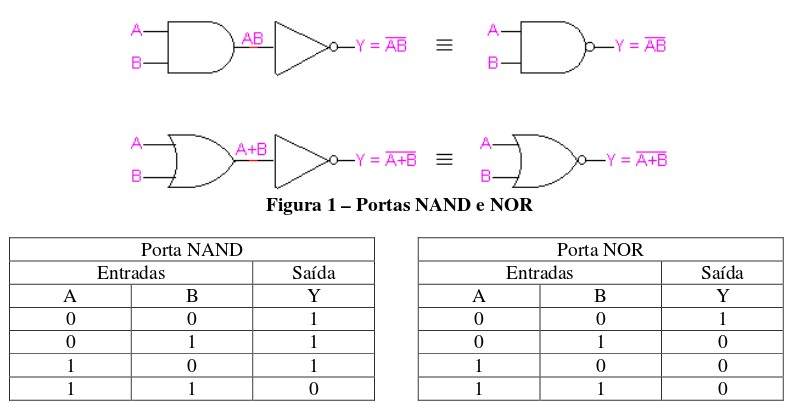
\includegraphics[width=.5\textwidth]{nandnor.jpg}
	\caption{Portas NAND e NOR}
	\label{fig:exemplo}
\end{figure}

Além das portas NAND e NOR, existem outras portas que, apesar de não serem universais tem aplicação muito útil: as portas XOR e XNOR. A primeira porta é conhecida como OU-exclusivo. Ela compara dois bits e a saída será 1 se e somente se os bits forem diferentes. Se houver mais de duas entradas, aí será 1 se houver um numero ímpar de valores verdadeiros com entrada. Já a porta XNOR, que produz a tabela verdae complementar da porta XOR, irá ter saída 1 quando as duas entradas forem iguais, ou, para o caso de mais de duas entradas, quando o número de entradas 1 for par. 

\begin{figure}[H]
	\centering
	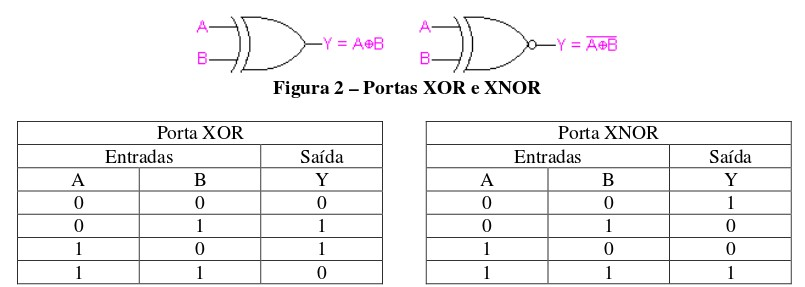
\includegraphics[width=.5\textwidth]{xorxnor.jpg}
	\caption{Portas XOR e XNOR}
	\label{fig:exemplo}
\end{figure}

A expressão dasportas XOR e XNOR podem ser escritas em termos das portas AND, OR e NOT:
A$\oplus$B = (NOT A . B) + (NOT B . A)
NOT(A $\oplus$ B) = (AB) + (NOT A . NOT B)


\subsection{ Fatores de Carga (fan-in, fan-out):}

O tempo de chaveamento de uma porta lógica depende do número de portas alimentadas pela saída. O Fan-out de uma porta é o número de portas que pode ser alimentado na saída e depende de como a porta é utilizada na sequência lógica. Ele representa o número máximo de entradas lógicas que uma saída pode acionar com segurança. Se o valor estabelecido pelo FAN-OUT for excedido, a tensão de nível lógico de saída não poderá ser mais garantida. Este conceito se aplica quando ocorre o consumo de energia das portas ligadas na saída. Seu valor depende da tecnologia empregada: 

• TTL: 2 a 10 
• CMOS: 50 a 100

Além disso, o termo Fan-in é utilizado para representar o número máximo de entradas que uma porta lógica possui. Para a para a série TTL 74XX, utilizada nos experimentos da matéria, tem-se: 

1 unidade de carga TTL = 40 $\mu$A, no nível lógico 1. 
= 1,6 mA, no nível lógico 0. 

Em outras palavras, uma porta 7400 que necessite de uma corrente de entrada máxima de IIL = 1,6 mA para o nível lógico 0 e uma corrente de entrada máxima IIH = 40 $\mu$A para o nível lógico 1 é especificada como tendo um fator de carga unitário. Isto é, possui um fan-in de 1. Por outro lado, a saída de uma porta 7400 absorverá 16 mA no nível lógico 0 e fornecerá 800 $\mu$A no nível lógico 1. Portanto, ela tem capacidade de acionar 10 portas no nível lógico 0 (pois 16 mA / 1,6 mA = 10). Isto é, possui um fan-out de 10 para o nível lógico 0. Da mesma forma, o fan-out para o nível lógico 1 é 800 $\mu$A / 40 $\mu$A = 20.


\subsection{Teorema de De Morgan:}

Um teorema muito útil e que comprova a universalidade de certos conjuntos de portas é o teorema de DeMorgan. Este teorema estabelece que:

\begin{enumerate}
	\item $\overline{A}$ + $\overline{B}$ = $\overline{A.B}$
	\item $\overline{A}$ . $\overline{B}$ = $\overline{A+B}$
\end{enumerate}

Isso, em outras palavras, quer dizer que, para retirar a negação de uma expressão devemos negar as partes e intercambiar a expressão entre elas. A partir disso é possível concluir o porque da universalidade das portas NAND e NOR. Nessas portas temos uma expressão negada, ou seja, é possivel criar variáveis negadas e obter a expressão lógica não originalmente testada pela porta. Para as portas NAND temos a seguinte relação:

\begin{figure}[H]
	\centering
	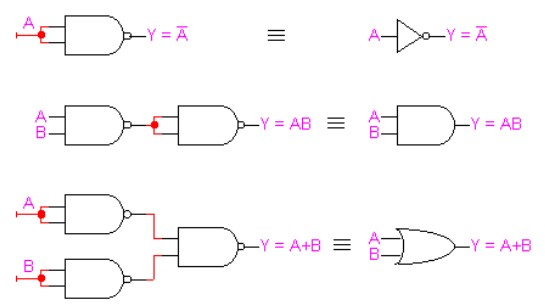
\includegraphics[width=.5\textwidth]{portanand.jpg}
	\caption{Universalidade da porta NAND}
	\label{fig:exemplo}
\end{figure}

Já para a porta NOR, temos:

\begin{figure}[H]
	\centering
	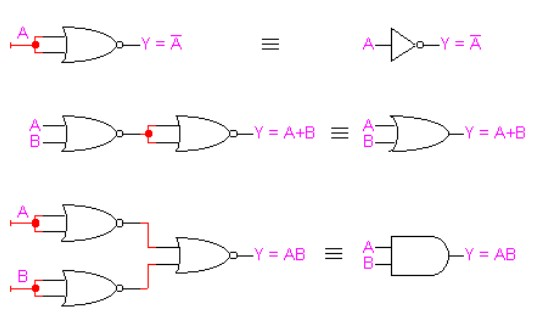
\includegraphics[width=.5\textwidth]{portanor.jpg}
	\caption{Universalidade da porta NOR}
	\label{fig:exemplo}
\end{figure}

Neste experimento iremos provar que esta universalidade é de fato verdadeira, e iremos explorar o funcionamento das portas NAND, NOR e XOR.



\section{Procedimentos}
\label{sec:Procedimentos}

\begin{itemize}
	\item Na primeira parte do experimento, foi implementado uma porta NAND de três entradas, utilizando-se três portas NAND de duas entradas:
	
	\begin{figure}[H]
		\centering
		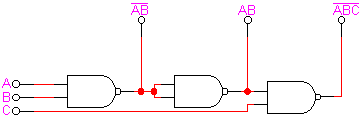
\includegraphics[width=.5\textwidth]{portanand3.jpg}
		\caption{Esquema da porta NAND de três entradas}
		\label{fig:exemplo}
	\end{figure}
	
	Após a devida implementação do circuito, foi preenchida a tabela da verdade para as saídas 
	$\overline{A.B}$, A.B e $\overline{A.B.C}$ imagem abaixo apresenta o circuito montado:
	
	\begin{figure}[H]
		\centering
		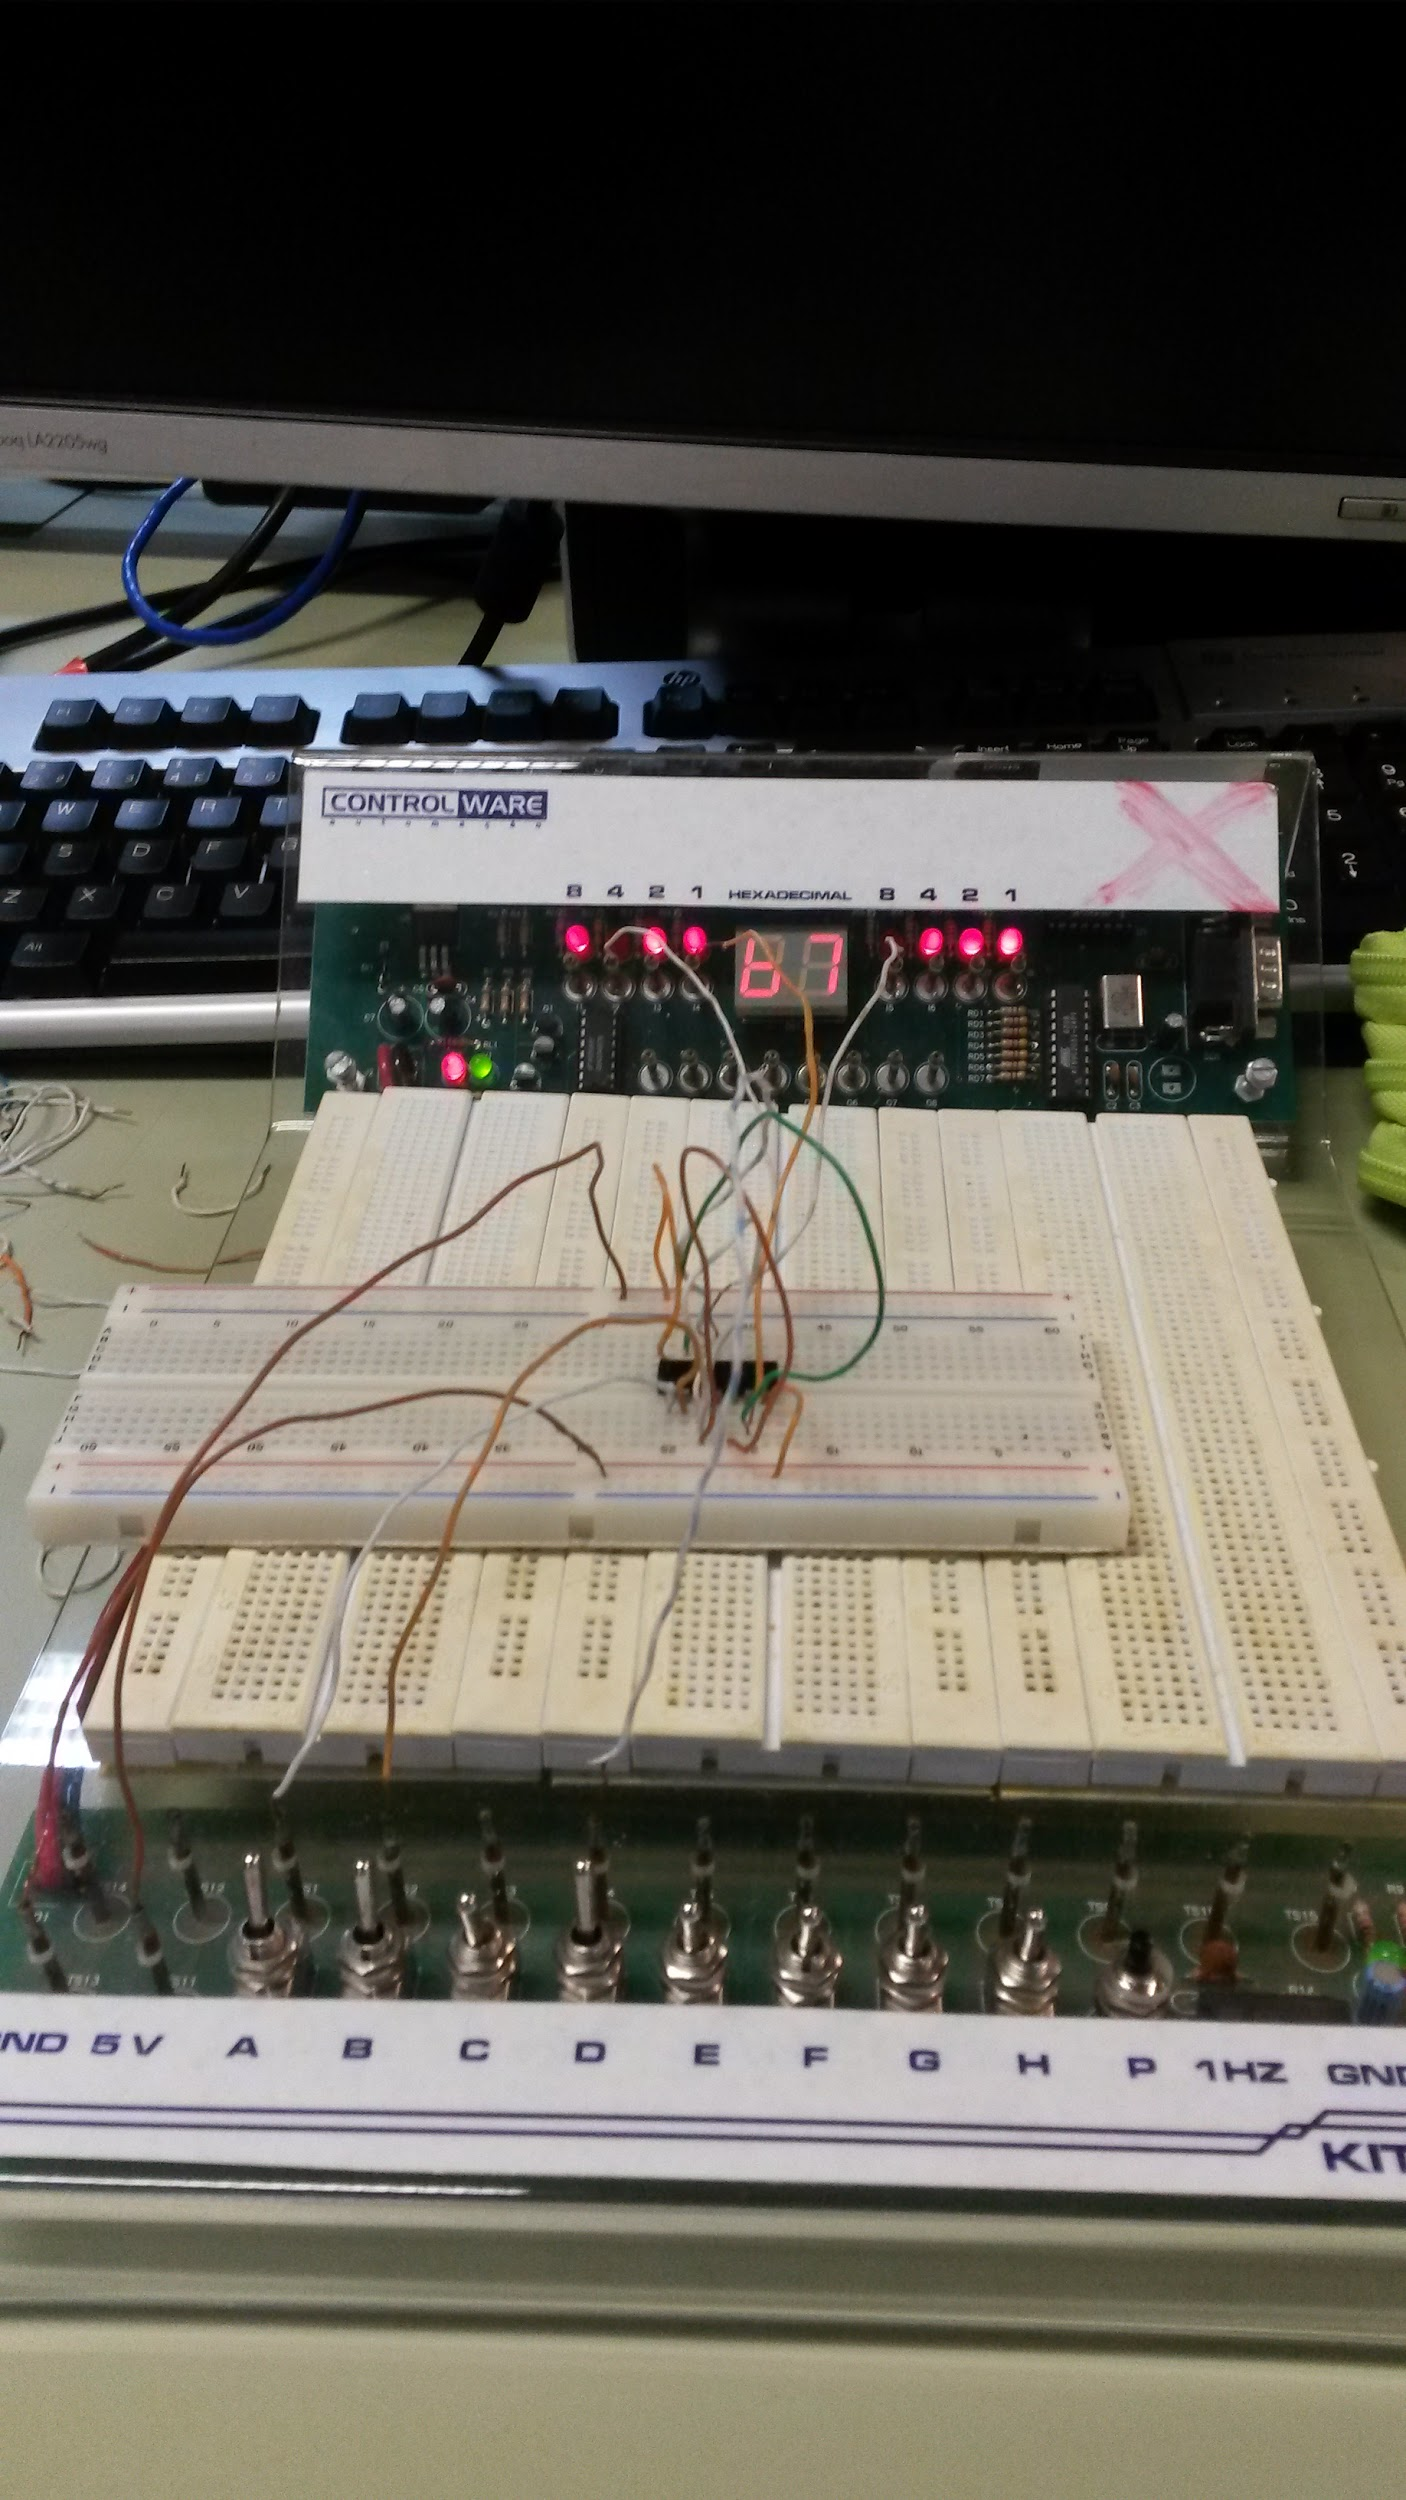
\includegraphics[width=.5\textwidth]{circuitonand.jpg}
		\caption{Porta NAND de três entradas}
		\label{fig:exemplo}
	\end{figure}
	
	\item Na segunda parte do experimento, implementou-se uma função XOR mediante a utilização de quatro portas NAND:
	
		\begin{figure}[H]
			\centering
			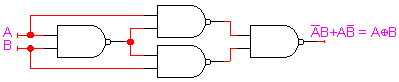
\includegraphics[width=.5\textwidth]{xor4.jpg}
			\caption{Esquema da função XOR com portas NAND.}
			\label{fig:exemplo}
		\end{figure}
	
	Após a devida implementação do circuito, foi preenchida a tabela verdade correspondente à função XOR.
	
	\begin{figure}[H]
		\centering
		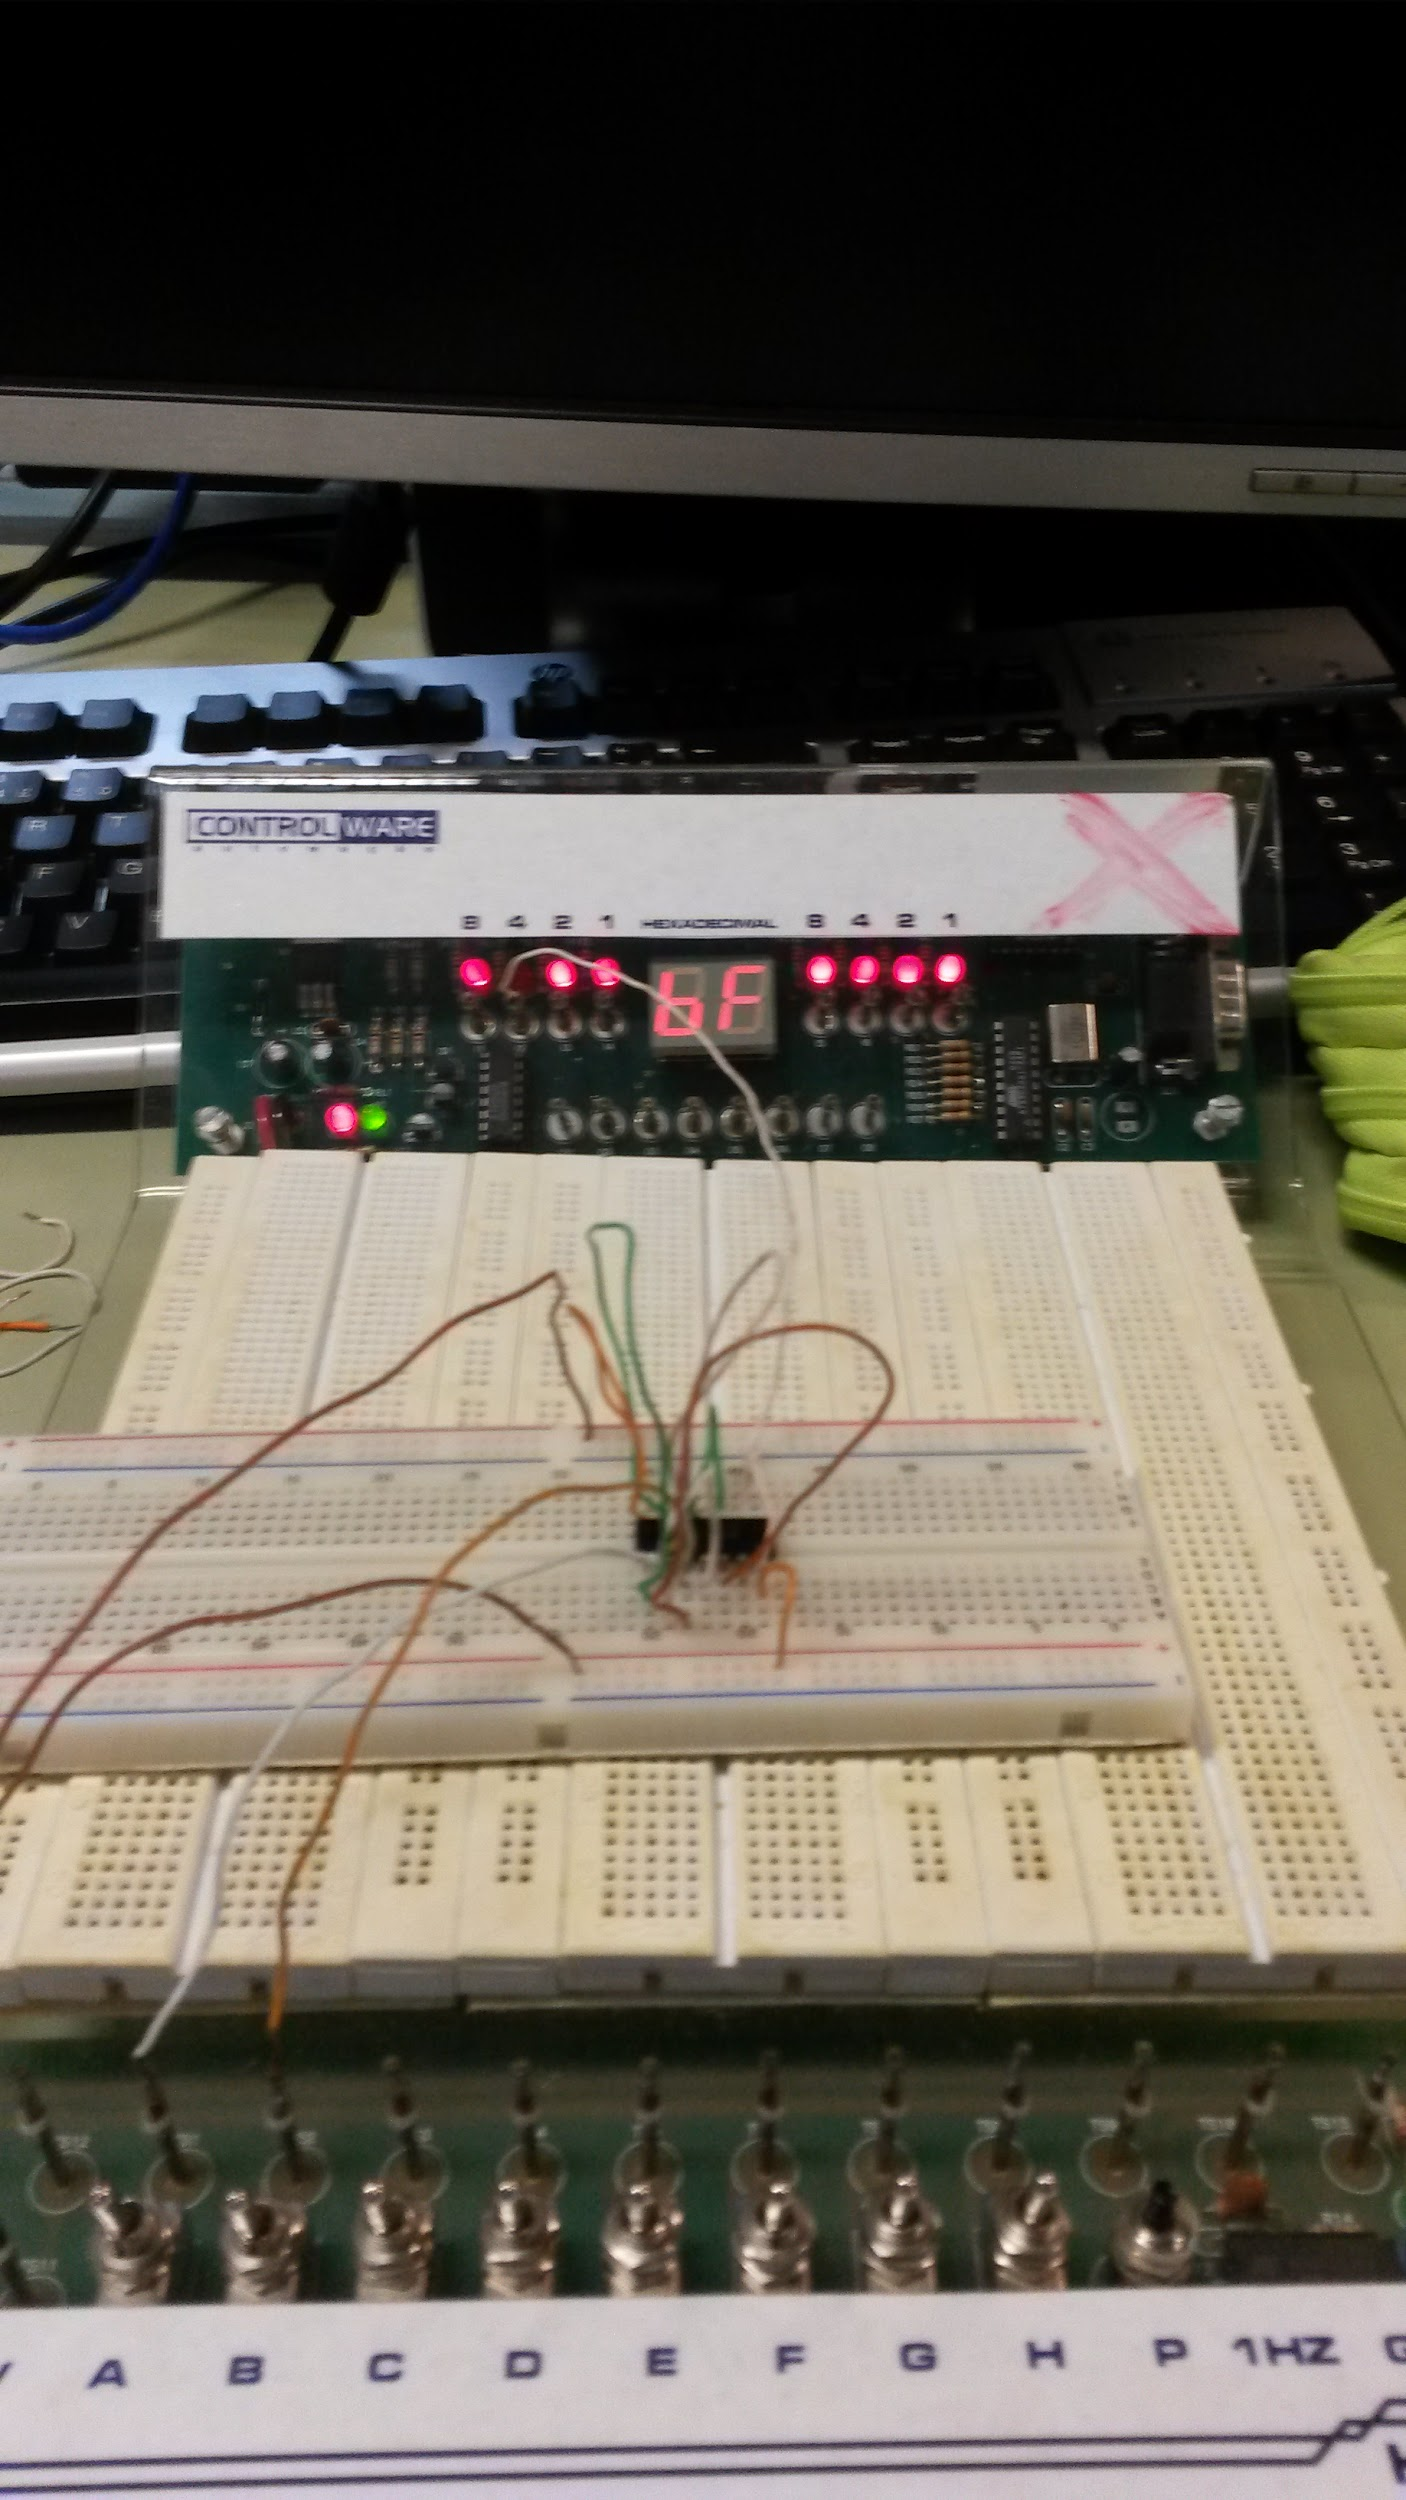
\includegraphics[width=.5\textwidth]{circuitoxor.jpg}
		\caption{Função XOR com portas NAND.}
		\label{fig:exemplo}
	\end{figure}
	
	\item Na última parte do experimento, uma porta XOR de quatro entradas foi projetada e implementada a partir da utilização de três portas XOR de duas entradas.
	
	\begin{figure}[H]
		\centering
		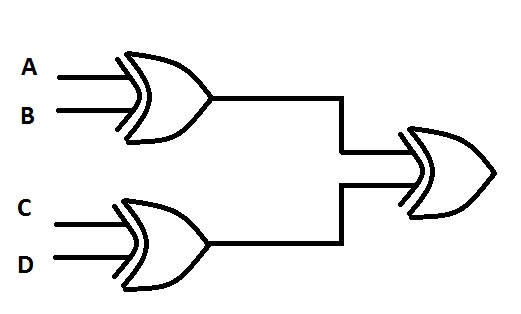
\includegraphics[width=.5\textwidth]{xor2.jpg}
		\caption{Função XOR de quatro entradas.}
		\label{fig:exemplo}
	\end{figure}
	
	Após a devida projeção e implementação do circuito, foram verificados os casos nos quais a saída do circuito corresponde a 1.
	
	\begin{figure}[H]
		\centering
		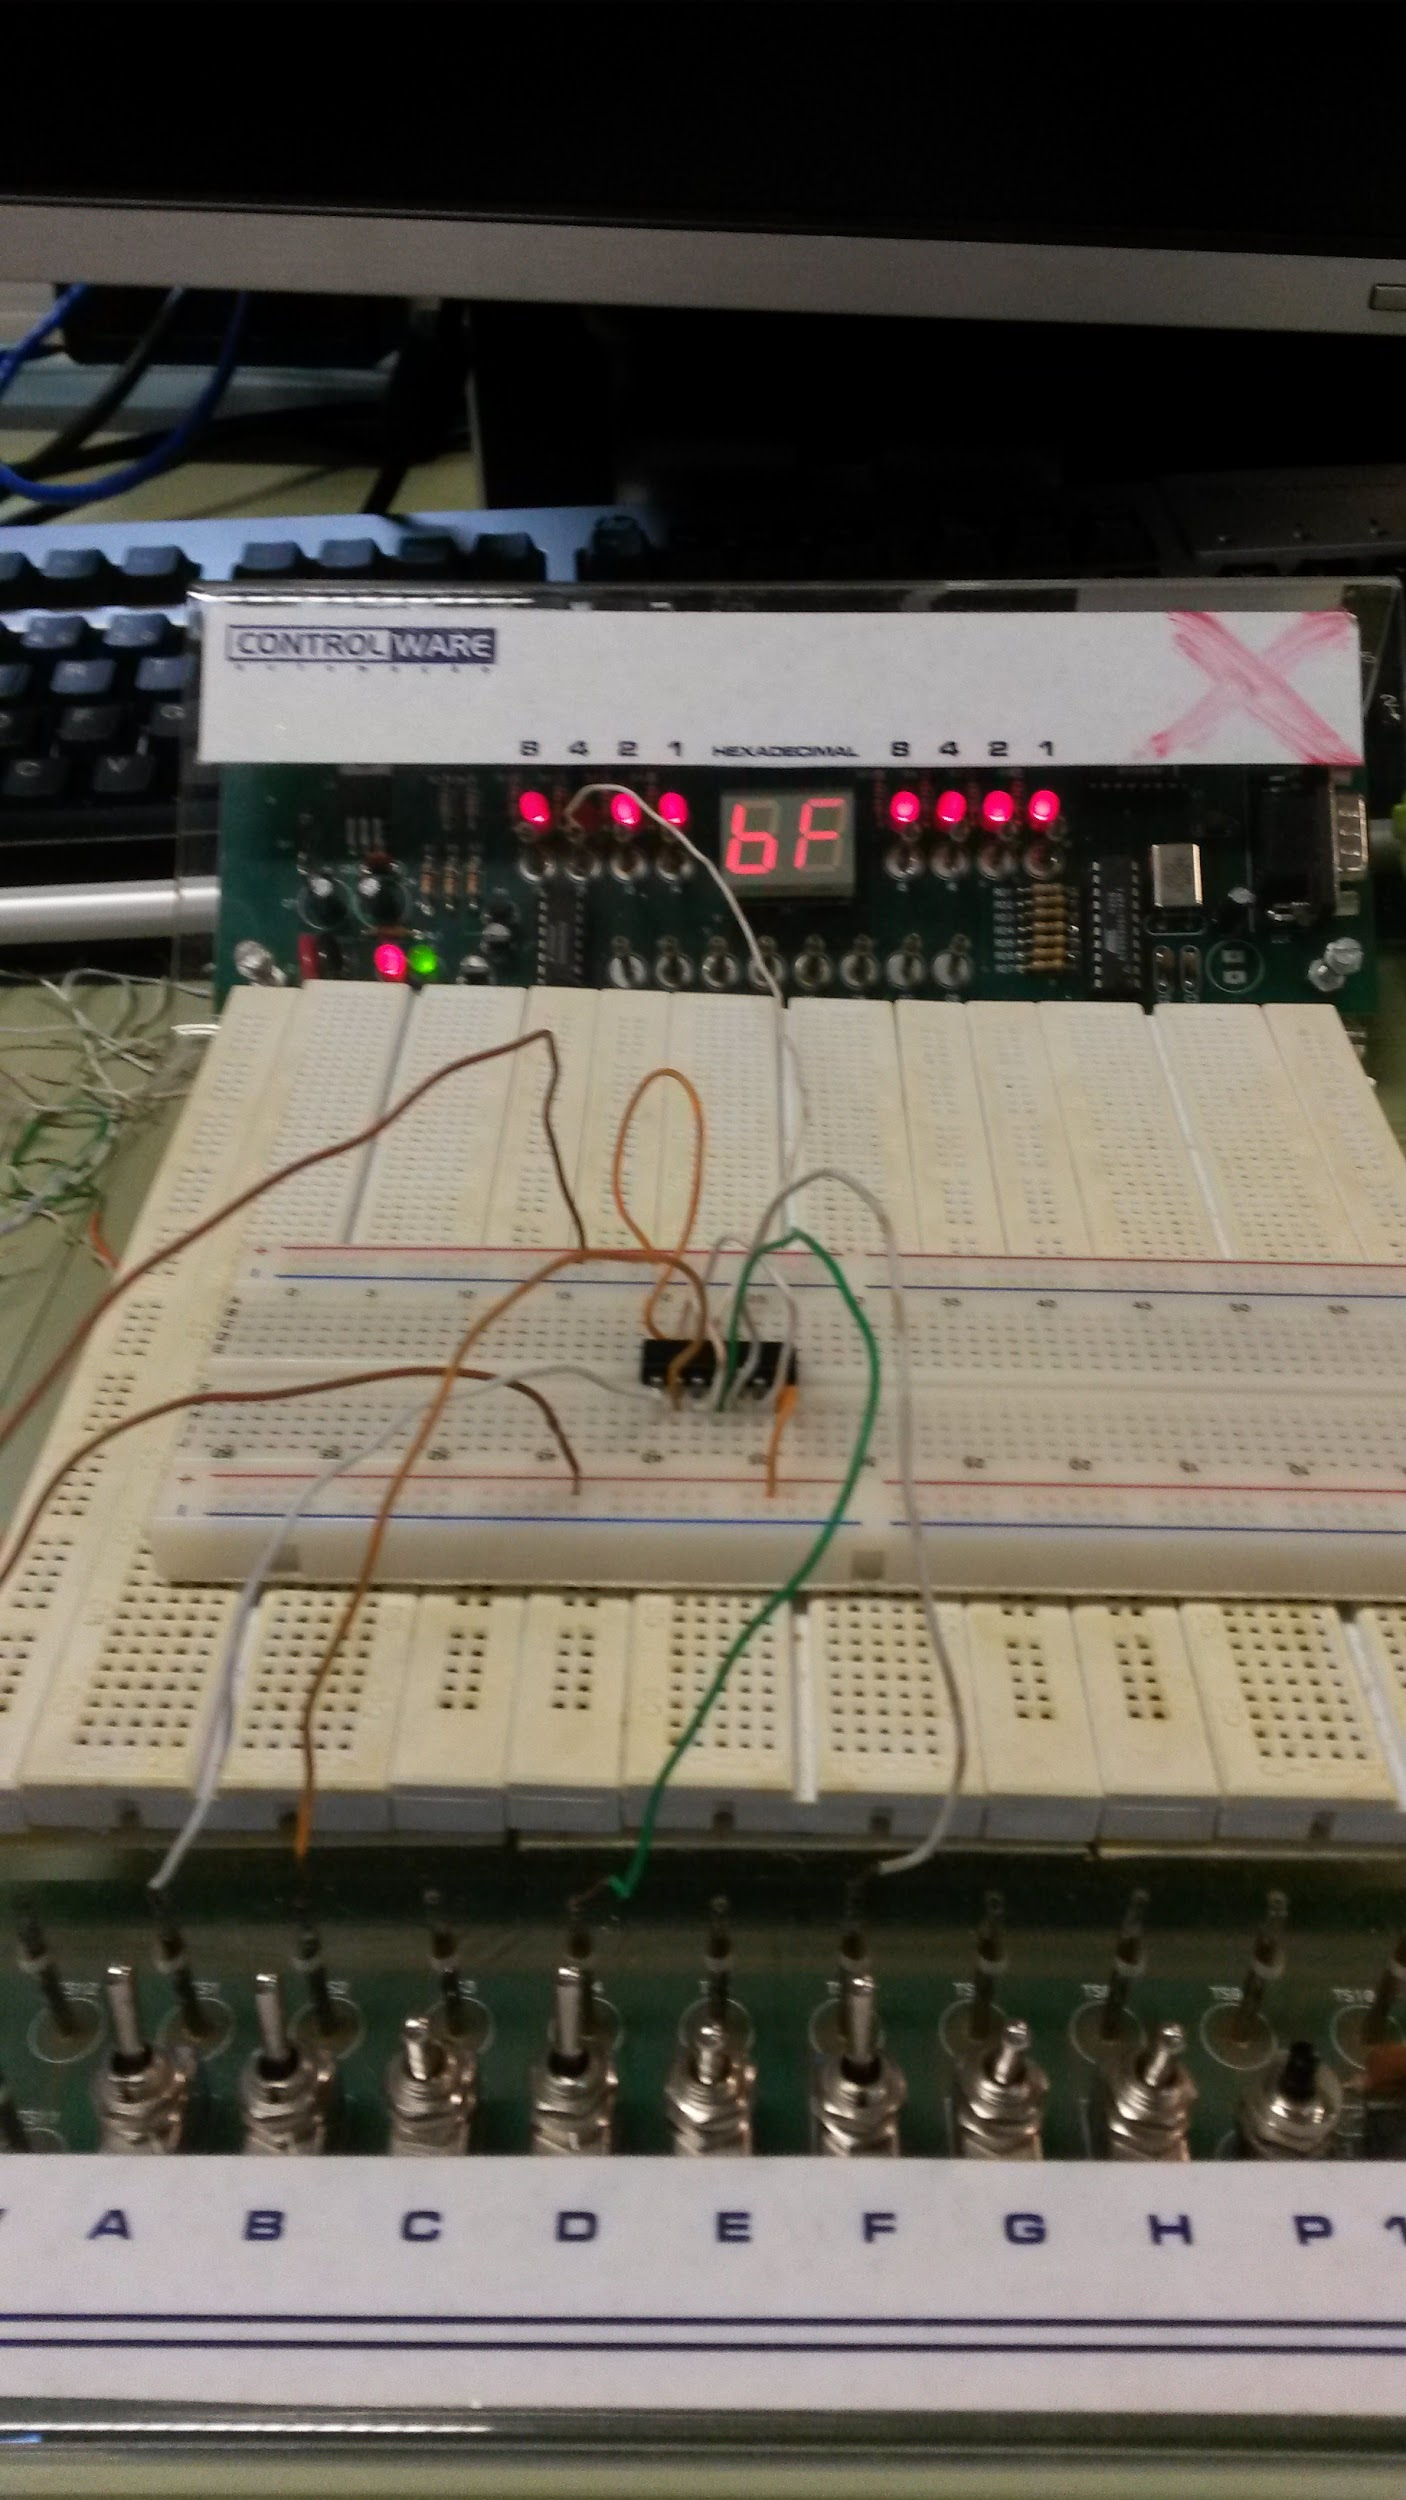
\includegraphics[width=.5\textwidth]{circuitoxor2.jpg}
		\caption{Função XOR com 4 entradas.}
		\label{fig:exemplo}
	\end{figure}
	
\end{itemize}
 
\subsection{Implementação de uma porta NAND de 3 entradas.}
\label{sec:NAND}

\begin{table}[H]
	\centering
	\begin{tabular}{|c|c|c|c|c|c|c|c|}
		\cline{1-6}
		\caption{Tabela verdade de uma porta NAND de 2 entradas, de uma porta NAND negada e te uma porta NAND de 3 entradas}
		\multicolumn{1}{|c|}{A} & \multicolumn{1}{|c|}{B} & \multicolumn{1}{|c|}{C} & \multicolumn{1}{|c|}{$\overline{A.B}$} & \multicolumn{1}{|c|}{A.B} & \multicolumn{1}{|c|}{$\overline{A.B.C}$}\\
		\hline
		0 & 0 & 0 & 1 & 0 & 1\\
		0 & 0 & 1 & 1 & 0 & 1\\
		0 & 1 & 0 & 1 & 0 & 1\\
		0 & 1 & 1 & 1 & 0 & 1\\
		1 & 0 & 0 & 1 & 0 & 1\\
		1 & 0 & 1 & 1 & 0 & 1\\
		1 & 1 & 0 & 0 & 1 & 1\\
		1 & 1 & 1 & 0 & 1 & 0\\
		\hline
	\end{tabular}
	\label{Porta NAND}
\end{table}


\subsection{Implementação da função XOR usando portas NAND.}
\label{sec:XOR}

A tabela verdade obtida após a construção do circuito encontra-se abaixo:

\begin{table}[H]
	\centering
	\begin{tabular}{|c|c|c|c|}
		\cline{1-4}
		\caption{Tabela verdade de uma porta XOR de 2 entradas}
		\multicolumn{1}{|c|}{A} & \multicolumn{1}{|c|}{B} & \multicolumn{1}{|c|}{A(XOR)B} \\
		\hline
		 0 & 0 & 0 \\
		 0 & 1 & 1 \\
		 1 & 0 & 1 \\
		 1 & 1 & 0 \\
		\hline
	\end{tabular}
	\label{Porta NAND}
\end{table}

\subsection{Verificação da função XOR usando a porta XOR (CI7486)}

A tabela verdade obtida para esta parte do experimento foi a mesma obtida na parte 2.2 (acima).

\subsection{Implementação de uma porta XOR de 4 entradas usando portas XOR de 2 entradas (CI 74LS86).}
\label{XOR2}


\begin{table}[H]
	\centering
	\begin{tabular}{|c|c|c|c|c|c|c|}
		\cline{1-5}
		\caption{Tabela verdade de uma porta NAND de 2 entradas, de uma porta NAND negada e te uma porta NAND de 3 entradas}
		\multicolumn{1}{|c|}{A} & \multicolumn{1}{|c|}{B} & \multicolumn{1}{|c|}{C} & \multicolumn{1}{|c|}{D} & \multicolumn{1}{|c|}{f(A,B,C,D)}\\
		\hline
		0 & 0 & 0 & 0 & 0 \\
		0 & 0 & 0 & 1 & 1 \\
		0 & 0 & 1 & 0 & 1 \\
		0 & 0 & 1 & 1 & 0 \\
		0 & 1 & 0 & 0 & 1 \\
		0 & 1 & 0 & 1 & 0 \\
		0 & 1 & 1 & 0 & 0 \\
		0 & 1 & 1 & 1 & 1 \\
		1 & 0 & 0 & 0 & 1 \\
		1 & 0 & 0 & 1 & 0 \\
		1 & 0 & 1 & 0 & 0 \\
		1 & 0 & 1 & 1 & 1 \\
		1 & 1 & 0 & 0 & 0 \\
		1 & 1 & 0 & 1 & 1 \\
		1 & 1 & 1 & 0 & 1 \\
		1 & 1 & 1 & 1 & 0 \\
		\hline
	\end{tabular}
	\label{Porta NAND}
\end{table}





\section{Análise dos Resultados}
\label{sec:Resultados}

Para todas as partes deste experimento temos que os dados obtidos corresponderam ao esperado, sendo iguais aos resultados teóricos.
Para ambas a parte 2.1 e a parte 2.2 vemos a aplicação direta do Teorema de DeMorgan, já que é possível obter uma função AND e uma função OR (que compoe a função XOR) a partir de uma negação da função AND.
Para a parte 2.1 foi provado como a porta AND pode ser substituída por 2 portas NAND gerando a mesma tabela verdade. Temos:

f(A,B) = NOT(AB)
Aplicando outra porta NAND, usando f(A,B) para as duas entradas, ficamos com:
f(A,B) = NOT(NOT(AB) . NOT(AB) = NOT(NOT(AB))
De acordo com DeMorgan:
f(A,B) = NOT (NOT A + NOT B) = NOT NOT A . NOT NOT B
f(A,B) = AB
Chegando a esse ponto, foi possivel implementar uma porta NAND de três entradas, incluindo f(A,B) e uma nova chave C, finalmente chegando à:

g(A,B,C) = NOT(f(A,B) . C) = NOT(ABC)

Para a parte 2.2 foi comprovada novamente essa universalidade da porta NAND, com a construção de uma porta XOR sendo feita apenas com a utilização da negação de AND. Temos, incialmente:

f(A,B) = NOT(AB) 
Por DeMorgan, f(A,B) = NOT A + NOT B 
Pegando este resultado e adicionando-o a uma nova porta NAND junto com a chave A:
g(A, f(A,B)) = NOT ((NOT A + NOT B) . A) = NOT(A . NOT B) = NOT A + B
Para a outra porta, onde o resultado é inserido em uma porta NAND com a chave B, temos:
h(B, f(A,B)) = NOT ((NOT A + NOT B) . B) = NOT(B . NOT A) = NOT B + A
Finalmente, juntando h e g em uma última porta NAND, ficaremos com:

F(A,B) = NOT((NOT A + B)(NOT B + A)) = NOT(NOT A + B) + NOT(NOT B + A)
= (NOT NOT A . NOT B) + (NOT NOT B . NOT A) = (A . NOT B) + (B . NOT A)

Que nada mais é do que a função XOR. 

Finalmente, na parte 2.4 vemos como a presença de apenas duas portas não deve nos limitar a utilizar apenas duas portas, pois é possível utilizar vários circuitos de duas portas para reproduzir circuitos com mais portas. Com 3 portas XOR foi possível reproduzir o resultado de caso a porta tivesse 4 entradas. Temos que, para duas portas XOR:

f(A,B) = (A . NOT B) + (B . NOT A)
g(C,D) = (C . NOT D) + (C . NOT D)
Juntando f e g em uma última porta XOR, ficaremos com:
h(A,B,C,D) = (NOT((A . NOT B) + (B . NOT A)) .  (C . NOT D) + (C . NOT D)) + (NOT  (C . NOT D) + (C . NOT D) .  (A . NOT B) + (B . NOT A))

Simplificando esta expressão, ficaremos com a soma dos minitermos indicando os oito casos em que a saída do circuito será 1:

h(A,B,C,D) = ABD(NOT C) + ABC(NOT D) + (NOT A)(NOT B)(NOT C)D + (NOT A)(NOT B)(NOT D)C + CD(NOT A)B + CD(NOT B)A + (NOT C)(NOT D)(NOT A)B + (NOT C)(NOT D)(NOT B)A

É possível notar que, nesta simplificação, serão verdadeiros apenas os casos em que temos um número ímpar de entradas 1.


\section{Conclusão}
\label{sec:Conclusao}

Formos apresentados às portas NAND e XOR, pudemos fazer de ambas as partes a implementaçao das tabelas verdade. Além disso, verificamos o Teorema DeMorgan e a fundamentabilidade da porta NAND.



\bibliographystyle{sbc}
\bibliography{relatorio}


\newpage 
% Colocar aqui apenas as respostas dos itens da Auto-Avaliação
\section*{Auto-Avaliação}

\begin{enumerate}
    \item B
    \item A
    \item D
    \item D
    \item B
\end{enumerate}


\end{document}
